\section{Source-localization algorithm}
\label{s:algorithm}
Formulas for calculating the direction of arrival (DOA) of a signal from FDOA or TDOA measurements were given in equations \ref{eq:doa} and \ref{eq:doa_t}, respectively. If the receivers move, measurements are recorded for a second time step, and the DOA is recalculated, the intersection of these lines will provide an estimate for the emitter location. This simple algorithm (in 2D) is described more precisely below. A schematic of an example run is shown in figure \ref{fig:doa}.
\begin{framed}
\noindent\textbf{Input:}
\begin{itemize}
  \item Receiver data: Location and velocity for two time steps. Without loss of generality, assume the receivers are centered at the origin in time step 1, and centered at $(c_x,c_y)$ at timestep 2.
  \item FDOA measurements between all pairs of receivers of the same time step.
\end{itemize}
\textbf{Output:}
\begin{itemize}
  \item Estimate for emitter location, $\tilde{\mbf{x}}=[\tilde{x},\tilde{y}]^T.$
\end{itemize}
\vspace{1ex}
\begin{enumerate}
  \item Calculate DOA for time step 1 and time step 2 ($\hat{\mathbf{x}}^{(1)}=[\hat{x}^{(1)},\hat{y}^{(1)}]^T,\hat{\mathbf{x}}^{(2)}=[\hat{x}^{(2)},\hat{y}^{(2)}]^T$) using equation \ref{eq:doa}.
  \item Find the intersection of the lines generated by (1):
  \begin{align*}
    \tilde{x} =& \dfrac{c_y - \hat{y}^{(2)}c_x/\hat{x}^{(2)}}{\hat{y}^{(1)}/\hat{x}^{(1)}-\hat{y}^{(2)}/\hat{x}^{(2)}} \\
    \tilde{y} =& \frac{\hat{y}^{(1)}}{\hat{x}^{(1)}}\cdot\tilde{x}.
  \end{align*}
  \item Return $\tilde{\mbf{x}}.$
\end{enumerate}
\end{framed}

\begin{center}
  \begin{figure}[H]
    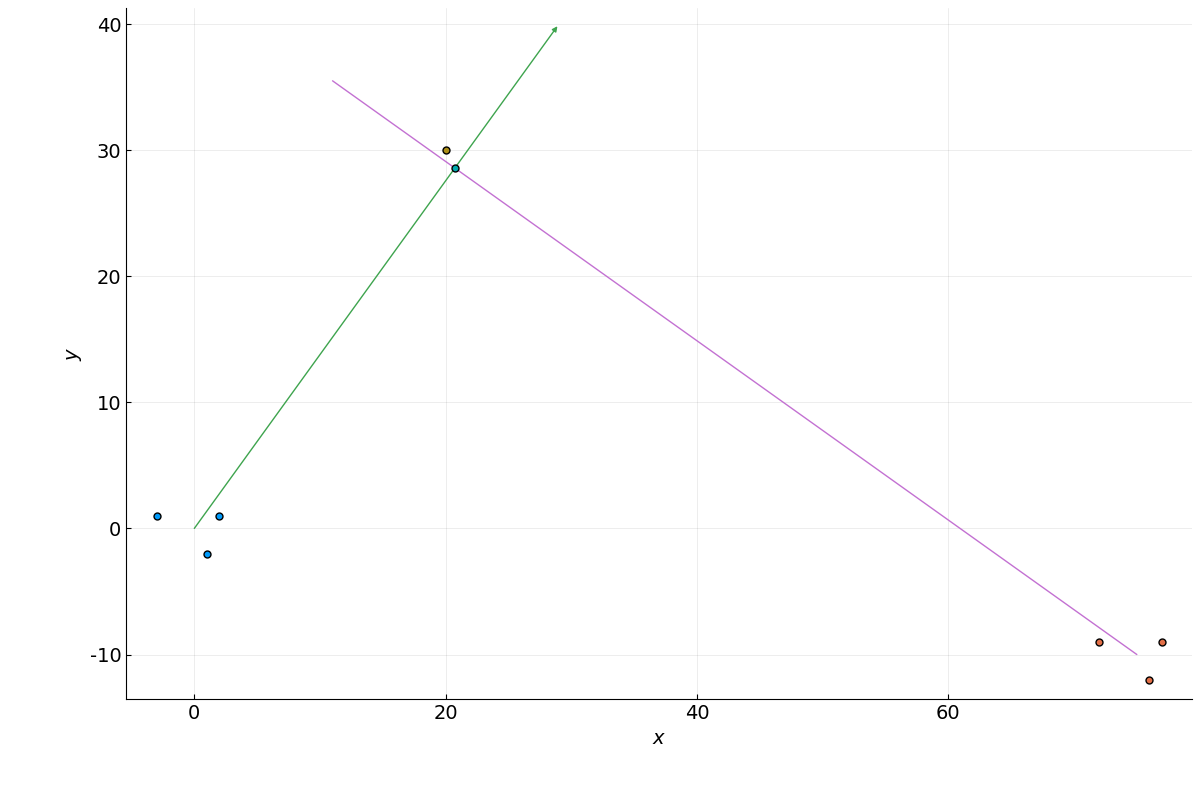
\includegraphics[scale=0.5]{DOA_proofofconcept}
    \caption{Proof of concept example for the proposed source localization algorithm in 2D with three receivers. In this example, the estimated location is $\tilde{\mbf{x}} = (20.7318,28.5771)$ and the correct location is $\mbf{x} = (20,30)$. The DOA calculations used FDOA measurements.}
    \label{fig:doa}
  \end{figure}
\end{center}
